% \iffalse meta-comment
%<*internal>
\iffalse
%</internal>
%<*readme>
----------------------------------------------------------------
pullquote --- make pullquotes with LaTeX
E-mail: Stephan.Lehmke@QuinScape.de
Web: www.docscape.de
Released under the LaTeX Project Public License v1.3c or later
See http://www.latex-project.org/lppl.txt
----------------------------------------------------------------

This package allows to insert an object between two columns of text.
%</readme>
%<*internal>
\fi
\def\nameofplainTeX{plain}
\ifx\fmtname\nameofplainTeX\else
  \expandafter\begingroup
\fi
%</internal>
%<*install>
\input docstrip.tex
\keepsilent
\askforoverwritefalse
\preamble
----------------------------------------------------------------
pullquote --- make pullquotes with LaTeX
E-mail: Stephan.Lehmke@QuinScape.de
Web: www.docscape.de
Released under the LaTeX Project Public License v1.3c or later
See http://www.latex-project.org/lppl.txt
----------------------------------------------------------------

\endpreamble
\postamble

Copyright (C) 2012 by Stephan Lehmke <Stephan.Lehmke@QuinScape.de>

This work may be distributed and/or modified under the
conditions of the LaTeX Project Public License (LPPL), either
version 1.3c of this license or (at your option) any later
version.  The latest version of this license is in the file:

http://www.latex-project.org/lppl.txt

This work is "maintained" (as per LPPL maintenance status) by
Stephan Lehmke.

This work consists of the file  pullquote.dtx
and the derived files           pullquote.ins,
                                pullquote.pdf, and
                                pullquote.sty.

\endpostamble
\usedir{tex/latex/pullquote}
\generate{
  \file{\jobname.sty}{\from{\jobname.dtx}{package}}
}
%</install>
%<install>\endbatchfile
%<*internal>
\usedir{source/latex/pullquote}
\generate{
  \file{\jobname.ins}{\from{\jobname.dtx}{install}}
}
\nopreamble\nopostamble
\usedir{doc/latex/demopkg}
\generate{
  \file{README.txt}{\from{\jobname.dtx}{readme}}
}
\ifx\fmtname\nameofplainTeX
  \expandafter\endbatchfile
\else
  \expandafter\endgroup
\fi
%</internal>
%<*package>
\NeedsTeXFormat{LaTeX2e}
\ProvidesPackage{pullquote}[2012/09/12 v2.0 EXPERIMENTAL package for typesetting pullquotes]
%</package>
%<*driver>
\documentclass{ltxdoc}
\usepackage[T1]{fontenc}
\usepackage{lmodern}
\usepackage{float}
\usepackage{tikz}
\usepackage{lipsum}
\usepackage{tabularx}
\usepackage{booktabs}
\usepackage[latin,english]{babel}
\usepackage{\jobname}

\makeatletter
\input{t1lmtt.fd}
\DeclareFontShape{T1}{lmtt}{m}{it}
     {<-> sub*lmtt/m/sl}{}

\DeclareRobustCommand\textequals{=}
\newcommand\ttarg[1]{\texttt{\meta{#1}}}
\newcommand\default[1]{\par\vspace{-2\baselineskip}\mbox{}\hfill
  Default: \textbf{#1}\par\medskip}
\newcommand\usageindex[1]
{%
  \@bsphack
  \HD@page@wrindex{#1\actualchar{\protect\ttfamily#1}\encapchar usage}%
  \@esphack
}
\newcommand\ttindex[1]
{%
  \@bsphack
  \HD@page@wrindex{#1\actualchar{\protect\ttfamily#1}}%
  \@esphack
}
\newcommand\pindex[1]
{%
  \@bsphack
  \HD@page@wrindex{#1\actualchar{\protect\ttfamily#1} \mbox{(package)}}%
  \HD@page@wrindex{packages:\levelchar#1\actualchar{\protect\ttfamily#1}}%
  \@esphack
}
\DeclareRobustCommand\package[1]{\texttt{#1}\pindex{#1}}

\newcommand\poindex[1]
{%
  \@bsphack
  \HD@page@wrindex{#1\actualchar{\protect\ttfamily#1} \mbox{(package option)}}%
  \HD@page@wrindex{package options:\levelchar#1\actualchar{\protect\ttfamily#1}}%
  \@esphack
}
\DeclareRobustCommand\packageoption[1]{\texttt{#1}\poindex{#1}}

\newcommand\eoindex[1]
{%
  \@bsphack
  \HD@page@wrindex{#1\actualchar{\protect\ttfamily#1} \mbox{(environment option)}}%
  \HD@page@wrindex{environment options:\levelchar#1\actualchar{\protect\ttfamily#1}}%
  \@esphack
}
\DeclareRobustCommand\environmentoption[1]{\texttt{#1}\eoindex{#1}}

\newcommand\dontsplit
{\@nobreaktrue\nopagebreak}

\renewcommand*\descriptionlabel[1]{\hspace\labelsep
                                \normalfont\bfseries\boldmath #1}

\makeatother

\usepackage[numbered]{hypdoc}
\definecolor{lstbgcolor}{rgb}{0.9,0.9,0.9} 
 
\usepackage{listings}
\lstloadlanguages{[LaTeX]TeX}
\lstset{breakatwhitespace=true,breaklines=true,language=TeX}
 
\usepackage{fancyvrb}

\renewcommand\topfraction{.9}
\renewcommand\bottomfraction{.5}
\renewcommand\textfraction{.1}
\renewcommand\floatpagefraction{.8}


\newfloat{Example}{hbtp}{loe}

\newenvironment{example}[2]
  {\def\excaption{#1}\def\exlabel{#2}%
    \VerbatimEnvironment
   \begin{VerbatimOut}[gobble=2]{example.out}}
  {\end{VerbatimOut}
   \begin{Example}
     \centering\parindent0pt
   \fbox{\begin{minipage}{.9\linewidth}
     \lstset{breakatwhitespace=true,breaklines=true,language=[LaTeX]TeX,basicstyle=\small\ttfamily,flexiblecolumns}
     \lstinputlisting[]{example.out}
   \end{minipage}}

   \fbox{\begin{minipage}{.9\linewidth}
     \footnotesize\parindent=1em
     \input{example.out}
   \end{minipage}}%

 \caption{\excaption}\label{\exlabel}
\end{Example}
}

\newenvironment{texcode}
{%
  \lstset{breakatwhitespace=true,breaklines=true,language=[LaTeX]TeX,basicstyle=\small\ttfamily,flexiblecolumns}
  \begin{lstlisting}
}
{%
  \end{lstlisting}
}

\newenvironment{quotecode}
{%
  \begin{quote}
  \begin{lrbox}{\pqbox}
    \begin{minipage}{\dimexpr\linewidth-2\fboxsep-2\fboxrule\relax}
}
{
  \end{minipage}
  \end{lrbox}
    \fbox{\usebox{\pqbox}}
  \end{quote}
}

\immediate\write18{makeindex -s gglo.ist -o pullquote.gls pullquote.glo}
\immediate\write18{makeindex -s gind.ist pullquote.idx}


\EnableCrossrefs
\CodelineIndex
\RecordChanges
\begin{document}
  \DocInput{\jobname.dtx}
  \PrintChanges
  \PrintIndex
\end{document}
%</driver>
% \fi
%
%
% \CharacterTable
%  {Upper-case    \A\B\C\D\E\F\G\H\I\J\K\L\M\N\O\P\Q\R\S\T\U\V\W\X\Y\Z
%   Lower-case    \a\b\c\d\e\f\g\h\i\j\k\l\m\n\o\p\q\r\s\t\u\v\w\x\y\z
%   Digits        \0\1\2\3\4\5\6\7\8\9
%   Exclamation   \!     Double quote  \"     Hash (number) \#
%   Dollar        \$     Percent       \%     Ampersand     \&
%   Acute accent  \'     Left paren    \(     Right paren   \)
%   Asterisk      \*     Plus          \+     Comma         \,
%   Minus         \-     Point         \.     Solidus       \/
%   Colon         \:     Semicolon     \;     Less than     \<
%   Equals        \=     Greater than  \>     Question mark \?
%   Commercial at \@     Left bracket  \[     Backslash     \\
%   Right bracket \]     Circumflex    \^     Underscore    \_
%   Grave accent  \`     Left brace    \{     Vertical bar  \|
%   Right brace   \}     Tilde         \~}
%
%
% \changes{1.0}{2012/09/06}{Converted to DTX file}
%
% \DoNotIndex{\newcommand,\newenvironment}
% \DoNotIndex{\def,\long,\edef,\xdef,\gdef,\let,\global}
% \DoNotIndex{\if,\ifnum,\ifdim,\ifcat,\ifmmode,\ifvmode,\ifhmode,%
%             \iftrue,\iffalse,\ifvoid,\ifx,\ifeof,\ifcase,\else,\or,\fi}
% \DoNotIndex{\box,\copy,\setbox,\unvbox,\unhbox,\hbox,%
%             \vbox,\vtop,\vcenter}
% \DoNotIndex{\@empty,\empty,\immediate,\write,\@tempdima,\@tempdimb,\@tempcnta,\@tmp}
% \DoNotIndex{\egroup,\bgroup,\expandafter,\begingroup,\endgroup}
% \DoNotIndex{\divide,\advance,\multiply,\count,\dimen}
% \DoNotIndex{\relax,\space,\string}
% \DoNotIndex{\csname,\endcsname,\@spaces,\openin,\openout,%
%             \closein,\closeout}
% \DoNotIndex{\catcode,\endinput}
% \DoNotIndex{\jobname,\message,\read,\the,\noexpand}
% \DoNotIndex{\hsize,\vsize,\hskip,\vskip,\kern,\hfil,\hfill,\hss}
% \DoNotIndex{\m@ne,\z@,\z@skip,\@ne,\tw@,\p@,\strip@pt}
% \DoNotIndex{\dp,\wd,\ht,\vss,\unskip}
% \DoNotIndex{\@nil,\do,\next,\repeat}
% \DoNotIndex{\ ,\vspace}
% \DoNotIndex{\dimexpr,\numexpr,\number}
% \tolerance9999
% \providecommand*{\url}{\texttt}
% \GetFileInfo{pullquote.dtx}
% \newsavebox\pqbox
% \makeatletter
% \gdef\tshortstack{\@ifnextchar[\@tshortstack{\@tshortstack[c]}}
% \gdef\@tshortstack[#1]{%
%   \leavevmode
%   \vtop\bgroup
%     \baselineskip-\p@\lineskip 3\p@
%     \let\mb@l\hss\let\mb@r\hss
%     \expandafter\let\csname mb@#1\endcsname\relax
%     \let\\\@stackcr
%     \@ishortstack}
% \makeatother
% \title{The \textsf{pullquote} package}
% \author{Stephan Lehmke \\ \url{mailto:Stephan.Lehmke@QuinScape.de} \\ \url{www.docscape.de}}
% \date{\fileversion~from \filedate}
%
%
% \maketitle
%
% \begin{abstract}
%   A \emph{pull quote} (also known as a lift-out quote) is a
%   quotation or excerpt from an article that is typically placed in a
%   larger or distinctive typeface on the same page, serving to entice
%   readers into an article or to highlight a key topic (from
%   \href{http://en.wikipedia.org/wiki/Pull_quote}{Wikipedia}).
%
%   In journal publishing, where multi-column typesetting is common, a
%   pull quote is usually placed between two columns, inside a
%   `window' which is cut out of the columns' text flow. Pictures and
%   other graphical objects are also often placed this way.
%
%   This package implements an environment for typesetting a balanced
%   two-column text with a cut-out window of customizeable shape in
%   which an arbitrary object is positioned.
% \end{abstract}
%
% \tableofcontents
% 
% \listof{Example}{Examples}
%
% 
%     \def\alicetext
%     {%
%       \selectlanguage{english}%
%       They were indeed a queer-looking party that assembled on the bank--the birds with draggled feathers, the animals with their fur clinging close to them, and all dripping wet, cross, and uncomfortable.
%
%       The first question of course was, how to get dry again: they had a consultation about this, and after a few minutes it seemed quite natural to Alice to find herself talking familiarly with them, as if she had known them all her life. Indeed, she had quite a long argument with the Lory, who at last turned sulky, and would only say, `I am older than you, and must know better'; and this Alice would not allow without knowing how old it was, and, as the Lory positively refused to tell its age, there was no more to be said.
%
%       At last the Mouse, who seemed to be a person of authority among them, called out, `Sit down, all of you, and listen to me! I'll soon make you dry enough!' They all sat down at once, in a large ring, with the Mouse in the middle. Alice kept her eyes anxiously fixed on it, for she felt sure she would catch a bad cold if she did not get dry very soon.
%
%       `Ahem!' said the Mouse with an important air, `are you all ready? This is the driest thing I know. Silence all round, if you please! "William the Conqueror, whose cause was favoured by the pope, was soon submitted to by the English, who wanted leaders, and had been of late much accustomed to usurpation and conquest. Edwin and Morcar, the earls of Mercia and Northumbria--"'
%
%       `Ugh!' said the Lory, with a shiver.
%
%       `I beg your pardon!' said the Mouse, frowning, but very politely: `Did you speak?'
%
%       `Not I!' said the Lory hastily.
%
%       `I thought you did,' said the Mouse. `--I proceed. "Edwin and Morcar, the earls of Mercia and Northumbria, declared for him: and even Stigand, the patriotic archbishop of Canterbury, found it advisable--"'
%
%       `Found what?' said the Duck.
%     
%       `Found it,' the Mouse replied rather crossly: `of course you know what "it" means.'
%
%       `I know what "it" means well enough, when I find a thing,' said the Duck: `it's generally a frog or a worm. The question is, what did the archbishop find?'
%
%       The Mouse did not notice this question, but hurriedly went on, `"--found it advisable to go with Edgar Atheling to meet William and offer him the crown. William's conduct at first was moderate. But the insolence of his Normans--" How are you getting on now, my dear?' it continued, turning to Alice as it spoke.
% }
%
% \section{Introduction}
%
% This is an \emph{experimental} package for inserting an arbitrary
% object into a two-column balanced text flow such that a ``window''
% of appropriate size is cut out of the text at the place the object
% is inserted.
%
% Different window shapes are supported, for instance rectangular and
% circular shapes. New shapes can easily be added by providing a
% specific type of macro called \emph{shape function}.
%
% In its current state, the package is more like a proof of concept,
% demonstrating how this effect can be achieved by \TeX\ macro
% programming. For being really useful, there are too many
% restrictions at the time being. See sections \ref{sec:Requirements},
% \ref{sec:Limitations},
% and \ref{sec:Extensions}.
% \begin{figure}
%   \begin{lrbox}{\pqbox}
%     \begin{minipage}{\textwidth}
%       \begin{pullquote}
%       {%
%       object=%
%       {\begin{tabular}[b]{p{4cm}}
%         \midrule
%         \textit{Wir m\"ussen wissen.}\\
%         \textit{Wir werden wissen.}\\
%         \mbox{}\hfill\small\textsc{David Hilbert}\\
%         \midrule
%       \end{tabular}}%
%     }
%       \selectlanguage{latin}\lipsum[1-4]
%     \end{pullquote}
%   \end{minipage}
%   \end{lrbox}
%   \begin{minipage}[b]{\dimexpr.5\textwidth-3mm}
%     \resizebox{\linewidth}{!}{\usebox{\pqbox}}
%     \caption{Text with rectangular insert using \texttt{pullquote}.}
%     \label{fig:rectpq}
%   \end{minipage}\hfill
%   \begin{lrbox}{\pqbox}
%     \begin{minipage}{\textwidth}
%       \begin{pullquote}
%       {%
%       shape=circular,%
%       object=%
%       {%
%       \begin{tikzpicture}
%         \clip (0,0) circle (2.7cm);
%         \node (0,0) {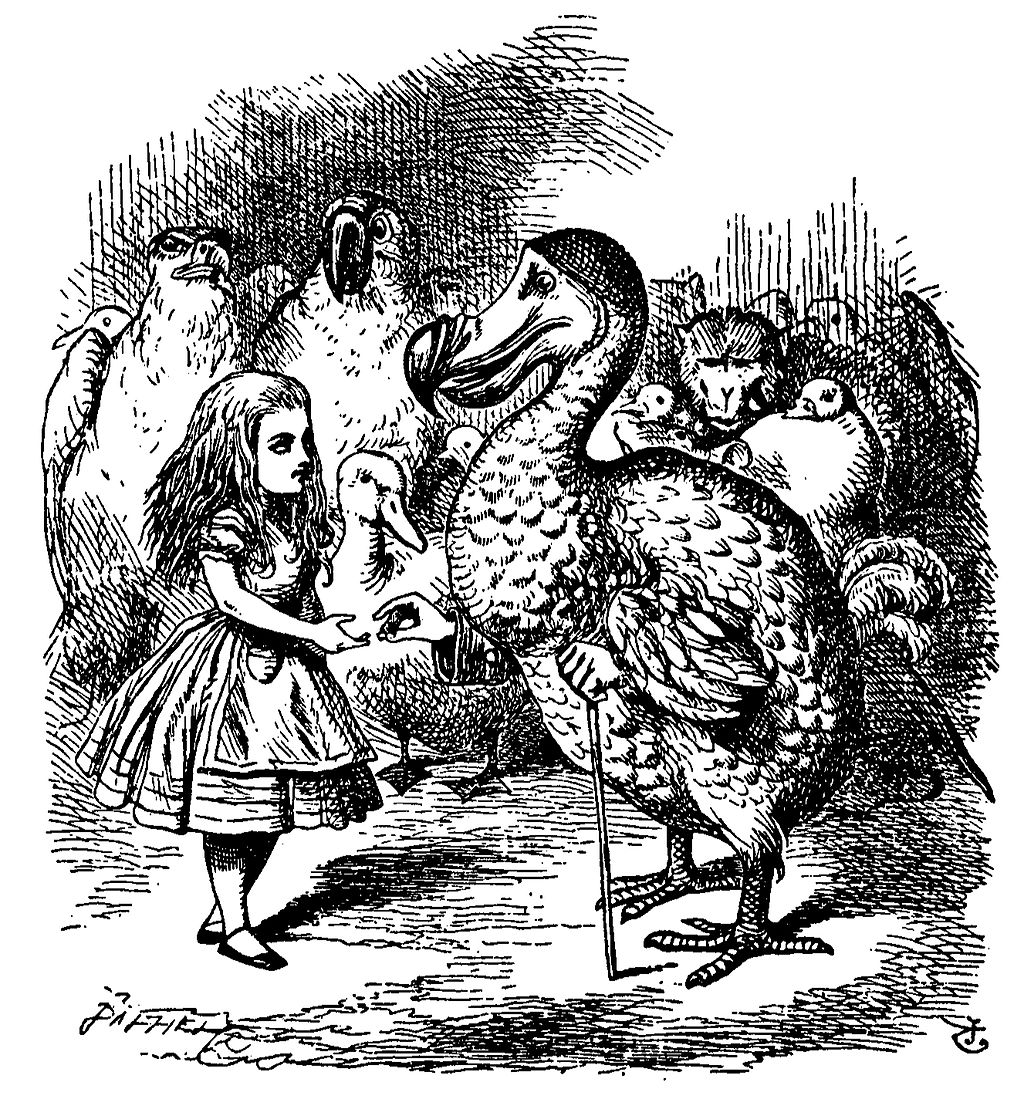
\includegraphics[width=5.2cm]{pq-alice}};
%       \end{tikzpicture}%
%       }
%     }
%       \alicetext
%     \end{pullquote}
%   \end{minipage}
%   \end{lrbox}
%   \begin{minipage}[b]{\dimexpr.5\textwidth-3mm}
%     \resizebox{\linewidth}{!}{\usebox{\pqbox}}
%     \caption{Text with circular insert using
%     \texttt{shape=circular}. Text and image by \textsc{Lewis Carroll} (pdf from \url{gasl.org}) [Public domain], via Wikimedia Commons.}
%     \label{fig:circpq}
%   \end{minipage}
%
%   \bigskip
%   \bigskip
%
%   \begin{lrbox}{\pqbox}
%     \begin{minipage}{\textwidth}
%       \begin{pullquote}{shape=image,image=pq-duck.pdf,imageopts={width=5cm}}\lipsum[1-3]
%       \end{pullquote}
%     \end{minipage}
%   \end{lrbox}
%   \begin{minipage}[b]{\dimexpr.5\textwidth-3mm}
%     \resizebox{\linewidth}{!}{\usebox{\pqbox}}
%     \caption{Text with insert based on image shape using
%     \texttt{shape=image}. Image by
%     \href{http://tex.stackexchange.com/users/3094/paulo-cereda}{Paulo Cereda}.}  
%     \label{fig:imgpq}
%   \end{minipage}
% \end{figure}
% 
% Figures \ref{fig:rectpq}--\ref{fig:imgpq} show some examples of
% the style of formatting possible with this package.
%
% You are invited to test this package and find useful applications
% for it, but please be prepared for unexpected failures.
%
% The package was implemented in the course of answering the questions
% \href{http://tex.stackexchange.com/questions/45958/implementing-a-pullquotes-algorithm-in-latex}{``Implementing
% a pullquotes algorithm in \LaTeX''} and
% \href{http://tex.stackexchange.com/questions/53073/two-column-text-with-circular-insert}{``Two-column
% text with circular insert''} on the
% \href{http://tex.stackexchange.com}{Q\&A site \TeX\ Stack
% Exchange}. Report bugs at \href{https://launchpad.net/tex-sx/}{the
% \TeX-SX Launchpad site}. There is also a
% \href{http://chat.stackexchange.com/rooms/409/from-answers-to-packages}{chatroom}
% dedicated to the \TeX-SX packages.
%
% As soon as the package is a bit more bug-free, basically documented
% and acceptably user-friendly, it will be prepared for publication on
% \href{http://www.ctan.org}{CTAN}. 
%
% \section{Requirements}\label{sec:Requirements}
%
% \subsection{Required Packages}
%
% The \package{pullquote} package automatically loads the following
% further packages:
% \begin{enumerate}
% \item \package{etoolbox}, \package{environ}, \package{keyval}. 
% \item \package{microtype} (only if the package option
% \packageoption{nomicrotype} is 
% \emph{not} given): The text formatting done by this package can get
% awfully `tight' when text flows around objects. \package{microtype}
% significantly improves typographic quality in these situations. Use
% the option \packageoption{nomicrotype} only if you want to load
% \package{microtype} yourself and 
% avoid option clashes.
% \item \package{graphicx} (only if the package option \packageoption{noimageshapes} is
% \emph{not} given): As the \texttt{pullquote} environment with the
% option \texttt{shape=image} executes a
% call to \cs{includegraphics} in the \package{graphicx} variant, this
% package is needed unless you explicitly deactivate that option.
% \end{enumerate}
% 
% \subsection{External Calls to Image Magick}\label{sec:Requirements:ImageMagick}
%
% The \texttt{pullquote} environment with the
% option \texttt{shape=image} will generate an external system
% call to the command \texttt{convert} from the image manipulation
% software \href{http://www.imagemagick.org/}{Image Magick}. The
% purpose of this call is to determine the \emph{shape} of an inserted
% image to get an appropriate `smooth' text flow around the image.
%
% This option doesn't make sense without that call, so to use this
% option, you need to fulfil the following requirements.
%
% \begin{enumerate}
% \item The software package  \href{http://www.imagemagick.org/}{Image
% Magick} should be installed on your computer such that the command
% \texttt{convert} can be called from a command shell. You can check
% whether your installation will work for the purposes of this package
% by pasting the following call into a command shell \textbf{all on
% one line}:
% \begin{verbatim}
%   convert pq-duck.pdf -resize 124.99362x123.20798! -bordercolor white
%   -border 10x10 -morphology Erode Disk:10.3 -resize 26x13!
%   -black-threshold 95% -monochrome pq-duck.pdf.pqshape.txt 
% \end{verbatim}
% (assuming you're in the installation directory of the pullquote
% package and the file \texttt{pq-duck.pdf} is present).
%
% You should get no error message and a non-empty text file
% \texttt{pq-duck.pdf.pqshape.txt} should be produced.
%
% \item The \texttt{shell-escape} feature of \texttt{(pdf)tex},
% enabling \TeX\ to execute system commands, should be activated. If
% you don't want to activate it in a global configuration file, you
% should call |pdflatex| with the |--shell-escape| option.
%
% If you have generated this documentation and the example text in figure
% \ref{fig:imgpq} flows around the image, then all is well.
% 
% \end{enumerate}
%
% If you don't meet these requirements or are not feeling secure when
% \TeX\ is calling external tools, then you can turn off the
% \texttt{shape=image} option by giving the \emph{package option}
% \packageoption{noimageshapes}.
%
% Even without the \texttt{shape=image} option, you can let text flow
% around the \emph{bounding box} of an image by using the default
% rectangular shape of the \texttt{pullquote} environment and giving
% an \cs{includegraphics} call as \texttt{object}.
%
% \subsubsection{Remarks on Ubuntu Linux}
%
% That's the system I'm testing with. Installing Image Magick should
% be as easy as typing
% \begin{verbatim}
%   apt-get install imagemagick
% \end{verbatim}
% or using some dedicated installation tool like \texttt{synaptic}. 
%
% I didn't have to configure anything special wrt.\
% \texttt{shell-escape}, though I'm not entirely sure why this is so\dots
%
% \subsubsection{Remarks on Windows}
%
% I am indebted to the user
% \href{http://tex.stackexchange.com/users/9237/speravir}{speravir}
% for providing the following comments on using \texttt{pullquote}
% with Windows.
%
% As I have no possibility to test on Windows myself, I did my best to
% translate it from German to English, but am otherwise providing this
% advice as-is. If you are getting good results in other ways, please
% report to me and I'll try to incorporate further advice.
%
% \bigskip
% 
% Image Magick needs to be installed on your system. Unfortunately,
% there is already a system command \texttt{convert.exe} for
% converting FAT-drives into NTFS-drives. So you need to make sure
% that after installation, \texttt{convert} from the Image Magick
% suite is found \emph{before} the system version of \texttt{convert}.
%
% \paragraph{Installation:}
% \begin{enumerate}
% \item Download the binary release from
% \url{http://www.imagemagick.org/}, ideally in the form of an
% \emph{Installer}.  The portable version will pose problems (see below).
% \item Install. It is important that the program inserts itself into
% the system path |%PATH%| \emph{in front of} the entry for
% |C:\Windows\system32| to make sure that a call to \texttt{convert}
% will call the program from the Image Magick suite.
% \item 
% This will not work with the portable version of Image Magick, so in
% that case the tool should be called via a batch file where the
% system path is set.
% \item 
% When using MiK\TeX-portable, the \emph{start batch} needs to be
% augmented. See the following answer on \TeX.SX:
% \begin{center}
%   \url{http://tex.stackexchange.com/questions/50911/using-miktex-portable-texmaker-and-asymptote-from-a-usb-drive/51110#51110}
% \end{center}
% The topic there was \emph{Asymptote}, but it's the same principle.
% \end{enumerate}
% 
% \bigskip
%
% When executing \TeX, the command line option |--enable-write18| (or
% the alias |--shell-escape|) has to be set. People using a \TeX-editor
% need to configure this in the appropriate place.
% 
% \section{Usage}
%
% \subsection{Package Options}
% Currently, there are only some simple options to pre-configure this package:
% \begin{description}
% \item[\packageoption{nomicrotype}] Normally, the \package{pullquote} package loads
% the package \package{microtype} which enhances typesetting in `tight
% places'. If you don't want to have this package loaded by
% \package{pullquote} because you don't want to use it or want to load
% it yourself, you can disable it by this package option.
%
% The package is not strictly neccessary for anything
% \texttt{pullquote} does, so apart from slightly worse typesetting
% quality, you won't notice anything when giving that option.
%
% \item[\packageoption{noimageshapes}] The option \texttt{shape=image} of the
% \texttt{pullquote} environment requires loading the package
% \package{graphicx} as well as the possibility to make an external
% system call to the software \href{http://www.imagemagick.org/}{Image
% Magick} (see section \ref{sec:Requirements:ImageMagick}).
%
% You can avoid all this by turning off this part of
% \package{pullquote} by giving this package option. Note that using
% the option \texttt{shape=image} will give an error message in this
% case. 
% \end{description}
% 
% \subsection{Basic Configuration}
%
% All of the configuration parameters for the \texttt{pullquote}
% environment can be specified by appropriate environment options; see
% section \ref{sec:Usage:Options}. Most of these options have
% \emph{canonical} defaults; for some of them you can specify default
% values by setting the following registers.
%
% \begin{description}
% \item[\cs{textcoldist}] \DescribeMacro{\textcoldist} The distance
% between the two text 
%   columns. Default for the option \texttt{textcoldist}. You can set
%   this register to 6mm by
% \begin{verbatim}
%   \setlength{\textcoldist}{6mm}
% \end{verbatim}
% \default{4mm}
%   
% \item[\cs{objdist}] \DescribeMacro{\objdist} The distance around the
% inserted object. Default 
%   for the option \texttt{objdist}. You can set
%   this register to 6mm by
% \begin{verbatim}
%   \setlength{\objdist}{6mm}
% \end{verbatim}
% \default{4mm}
% \end{description}
%
% \subsection{Basic Usage}\label{sec:Usage:Basic}
%
% To make a two-column text with a pull quote, you need
% \begin{itemize}
% \item some \emph{text}, which will be denoted by \ttarg{text} below and
% \item an \emph{object} to be inserted between the columns, denoted
% by \ttarg{object}. 
% \end{itemize}
% 
% Then creating the pull quote representation is as easy as
% calling\DescribeEnv{pullquote}\dontsplit 
%    \begin{quotecode}
%   |\begin{pullquote}{object=|\ttarg{object}|}|\\
%   \mbox{\quad}\ttarg{text}\\
%   |\end{pullquote}|
% \end{quotecode}
% 
% Example \ref{Ex:first} assumes you have loaded the package
% \package{lipsum} which provides a macro for \emph{blind text}.
% \begin{example}{Pull quote with tabular text \ttarg{object}.}{Ex:first}
%     \begin{pullquote}
%     {object=%
%       {%
%         \large\itshape
%         \begin{tabular}{@{}l@{}}
%           This is the\\pullquote text
%         \end{tabular}%
%       }%
%     }%
%       \selectlanguage{latin}\lipsum[1]
%     \end{pullquote}
% \end{example}
%
% In general, the \texttt{pullquote} environment is called like this:\dontsplit
%    \begin{quotecode}
%   |\begin{pullquote}{|\ttarg{options}|}|\\
%   \mbox{\quad}\ttarg{text}\\
%   |\end{pullquote}|
% \end{quotecode}
% 
% The content of the \texttt{pullquote} environment is just
% \ttarg{text}, while the \emph{mandatory argument} \ttarg{options} of
% the environment contains a comma-separated option list for
% configuring the appearance of the pull quote construction. It's
% similar to the \emph{key-value style} options which can be given to
% \cs{includegraphics} from the \package{graphicx} package, only here
% the argument is not optional because the \ttarg{object} always needs
% to be specified (usually with the \texttt{object} key, only in the
% special case of \emph{image shapes} you need to use the
% \texttt{image} key; see section \ref{sec:Usage:ImageShapes}). A full
% list of option keys and their use is described in section
% \ref{sec:Usage:Options}. 
%
% The use of \texttt{tabular} above is only one way of arranging text
% for use as \ttarg{object}. In fact, every \LaTeX\ construct of fixed
% \emph{width} and \emph{height} qualifies, for instance \cs{makebox},
% \cs{parbox} or \texttt{minipage}.
%
% Another typical choice for \ttarg{object} is an \emph{image}, like
% in example \ref{Ex:second}.
% \begin{example}{Pull quote with image \ttarg{object}.}{Ex:second}
%     \begin{pullquote}
%     {object={
\includegraphics[width=2cm]{pq-duck}}}%
%       \selectlanguage{latin}\lipsum[1]
%     \end{pullquote}
% \end{example}
% 
% Example \ref{Ex:options} shows some more options in use, with an object
% made by clipping an image with a circular path using Ti\textit{k}Z,
% a circular-shaped ``window'', an explicit \emph{vertical offset} and
% a slightly tighter distance between text and object than the usual
% default. The text by \textsc{Lewis Carroll} has been
% assigned to the macro \cs{alicetext}.
% \begin{example}{Pull quote with several options.}{Ex:options}
%     \begin{pullquote}
%     {%
%       shape=circular,objdist=2mm,objvoffset=3,%
%       object=%
%       {%
%         \begin{tikzpicture}
%           \clip (0,0) circle (1.7cm);
%           \node (0,0) {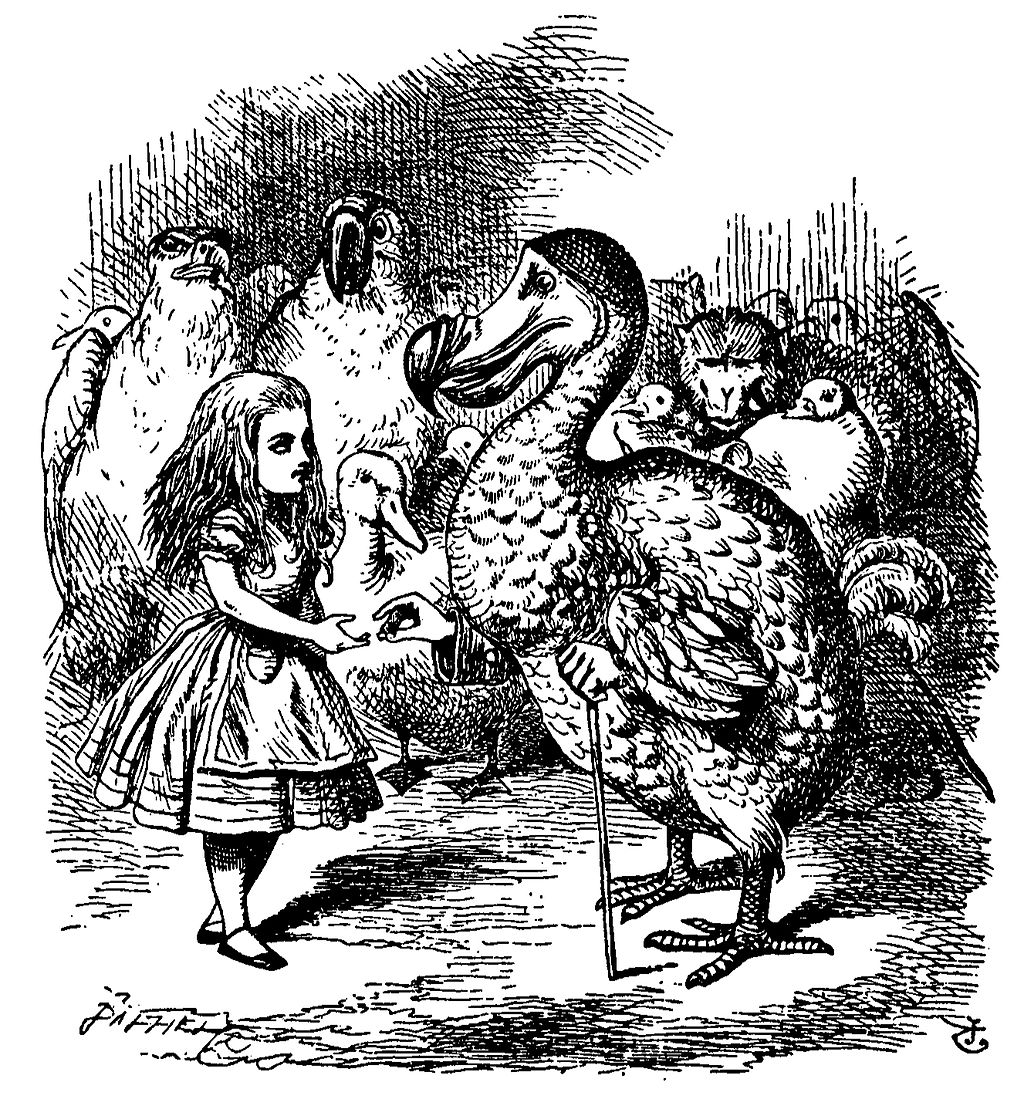
\includegraphics[width=3.2cm]{pq-alice}};
%         \end{tikzpicture}%
%       }
%     }
%       \alicetext
%     \end{pullquote}
% \end{example}
%
% \bigskip
%
% The \texttt{pullquote} environment is executed in the follwing steps:
% \begin{enumerate}
% \item Typeset \ttarg{object} into a \emph{box}, measuring its
%   \emph{width} and \emph{total height}.
% \item Add the value given by the option \texttt{objdist} (see
%   section \ref{sec:Usage:Options}) to the measured width and height
%   as a distance on all sides.
% \item \emph{Normalise} the height (including distance) to a full
%   number of text lines (measured in \cs{baselineskip}).
% \item The width and (normalised) height (including \texttt{objdist})
%   give the total size of the ``window'' to be cut out of the text
%   columns.
% \item Calculate the \emph{vertical position} of the window based on
%   its height and the value of the options \texttt{objvalign} or
%   \texttt{objvoffset}. 
% \item Calculate a \cs{parshape} definition for the surrounding
%   \ttarg{text} based on the size and position of the window.
% \item Typeset \ttarg{text} in two balanced columns according to the
%   pre-calculated \cs{parshape} definition. This may take several
%   attempts as it is impossible to estimate the exact number of lines
%   needed to typeset all text (and that number may even vary
%   depending on the exact `relative' position of the window and its
%   influence on paragraph formatting). The correct balance is
%   determined automatically by an internal loop.
% \item Arrange the balanced text columns with the object in the
%   predefined position to output the complete \emph{pull quote}
%   construct.
% \end{enumerate}
% 
% \bigskip
%
% Summary of remarks and restrictions on \ttarg{text}:
% \begin{itemize}
% \item \ttarg{text} should be just continuous text interspersed with
% \cs{par}. The result of typesetting \ttarg{text} in the given column
% width (using the predefined \cs{parshape} construct) is supposed to
% be a collection of plain text lines with base line distance
% \cs{baselineskip} (with the value in force at the beginning of the
% \cs{pullquote} environment). These lines are processed sequentially
% for calculating the \cs{parshape} construct and balancing the
% columns. 
% \item In particular, \ttarg{text} should \textbf{not} contain
% \begin{itemize}
% \item List environments like \texttt{itemize}, \texttt{quote} or
% \texttt{center}.
% \item Displayed math.
% \item Section headings.
% \item Any commands which change \cs{baselineskip}.
% \item Vertical spacing (or commands inserting it).
% \item Nothing which would make a line higher than usual text,
% which practically rules out \texttt{tabular} material.
% \item No fancy rules, frames or color tricks which can disturb 
% \cs{parshape} or vertical splitting of text.
% \end{itemize}
% Some of these restrictions may be loosened with future versions of
% the package; see sections \ref{sec:Limitations} and
% \ref{sec:Extensions}. 
% \end{itemize}
% 
%
%
%
%
% \subsection{Environment Options}\label{sec:Usage:Options}
% Remember the \texttt{pullquote} environment is called like this:
%    \begin{quotecode}
%   |\begin{pullquote}{|\ttarg{options}|}|\\
%   \mbox{\quad}\ttarg{text}\\
%   |\end{pullquote}|
% \end{quotecode}
% In this section, all the possible option keys which can go into
% \ttarg{options} are explained, together with their usage and
% interdependencies. 
%
% \begin{table}
%   \centering
%   \caption{Summary of Environment Options.}
%   \label{tab:optsummary}
%   \begin{tabularx}{\textwidth}{r>{\raggedright}Xll}
%     \toprule
%     \multicolumn{1}{l}{\textbf{Option}}&\textbf{Description}&\textbf{Default}&\textbf{P.}\\
%     \cmidrule(r){1-1}\cmidrule(rl){2-2}\cmidrule(rl){3-3}\cmidrule(l){4-4}\addlinespace
%     \environmentoption{textcoldist}&\texttt{=\meta{len}}\newline%
%     Distance between text columns.&%
%     \cs{textcoldist}&\pageref{eo:textcoldist}\tabularnewline\addlinespace
%     \environmentoption{objdist}&\texttt{=\meta{len}}\newline%
%     Distance inserted all around \ttarg{object}.&%
%     \cs{objdist}&\pageref{eo:objdist}\tabularnewline\addlinespace
%     \environmentoption{textcolwd}&\texttt{=\meta{len}}\newline%
%     Width of one text column.&%
%     $\frac{1}{2}\left(\footnotesize\begin{array}{@{}l@{}}\cs{linewidth}-{}\\\ttarg{textcoldist}\end{array}\right)$&\pageref{eo:textcolwd}\tabularnewline\addlinespace\midrule\addlinespace%
%     \environmentoption{object}&\texttt{=\meta{object}}\newline%
%     Object to be inserted between text columns.&%
%     \textit{mandatory}&\pageref{eo:object}\tabularnewline\addlinespace
%     \environmentoption{image}&\texttt{=\meta{file name}}\newline%
%     Sets \ttarg{object} to be \texttt{\cs{includegraphics}\marg{file
%     name}}.&%
%     ---&\pageref{eo:image}\tabularnewline\addlinespace
%     \environmentoption{imageopts}&\texttt{=\meta{opts}}\newline%
%     \cs{includegraphics} options in conjunction with
%     \environmentoption{image} key.&%
%     ---&\pageref{eo:imageopts}\tabularnewline\addlinespace\midrule\addlinespace%
%     \environmentoption{objvalign}&\texttt{=(top\string|middle\string|center\string|bottom)}\newline
%     \emph{Vertical alignment} of the ``object window''.&%
%     \texttt{middle}&\pageref{eo:objvalign}\tabularnewline\addlinespace
%     \environmentoption{objvoffset}&\texttt{=\meta{offset}}\newline%
%     \emph{Vertical offset} of the ``object window''.&%
%     ---&\pageref{eo:objvoffset}\tabularnewline\addlinespace\midrule\addlinespace%
%     \environmentoption{shape}&\texttt{=(rectangular\string|circular\string|image)}\newline%
%     \emph{Shape} of the ``object window''.&%
%     \texttt{rectangular}&\pageref{eo:shape}\tabularnewline\addlinespace%
%     \environmentoption{shapefunction}&\texttt{=\meta{cs}}\newline%
%     \emph{Shape function}.&%
%     ---&\pageref{eo:shapefunction}\tabularnewline\addlinespace%
%     \bottomrule
%   \end{tabularx}
%   
% \end{table}
%
% Table \ref{tab:optsummary} on page \pageref{tab:optsummary} gives a
% summary of all options.
%
% \subsubsection{Geometry Configuration}
% \begin{description}
% \item[\environmentoption{textcoldist}\texttt{=\meta{len}}\phantomsection\label{eo:textcoldist}] sets the distance between
% text columns produced by \texttt{pullquote} to \ttarg{len}. To
% change the distance to 5mm, use 
% \begin{verbatim}
%   textcoldist=5mm
% \end{verbatim}
% \default{\cs{textcoldist}}
% Compare example \ref{Ex:first} with example \ref{Ex:textcoldist}.
% \begin{example}{\texttt{textcoldist} example.}{Ex:textcoldist}
%     \begin{pullquote}
%     {textcoldist=1cm,%
%      object=%
%       {%
%         \large\itshape
%         \begin{tabular}{@{}l@{}}
%           This is the\\pullquote text
%         \end{tabular}%
%       }%
%     }%
%       \selectlanguage{latin}\lipsum[1]
%     \end{pullquote}
% \end{example}
% 
% \item[\environmentoption{objdist}\texttt{=\meta{len}}\phantomsection\label{eo:objdist}] sets the distance inserted all
% around \ttarg{object} to \ttarg{len}. Note that the vertical
% distance can be slightly larger because it needs to be
% \emph{normalised} so that the ``window'' takes a full number of
% text lines.
%
% To
% change the distance to 5mm, use 
% \begin{verbatim}
%   objdist=5mm
% \end{verbatim}
% \default{\cs{objdist}}
% Compare example \ref{Ex:first} with example \ref{Ex:objdist}.
% \begin{example}{\texttt{objdist} example.}{Ex:objdist}
%     \begin{pullquote}
%     {objdist=1mm,%
%      object=%
%       {%
%         \large\itshape
%         \begin{tabular}{@{}l@{}}
%           This is the\\pullquote text
%         \end{tabular}%
%       }%
%     }%
%       \selectlanguage{latin}\lipsum[1]
%     \end{pullquote}
% \end{example}
% 
% \item[\environmentoption{textcolwd}\texttt{=\meta{len}}\phantomsection\label{eo:textcolwd}] sets the width of one text
% column to \ttarg{len}. If this option is not given, then the default
% value
% \begin{displaymath}
%   \frac{1}{2}\left(\cs{linewidth}-\ttarg{textcoldist}\right)
% \end{displaymath}
% is calculated in the moment the \texttt{pullquote} environment is
% executed, so the then-current value of \cs{linewidth} is respected.
%
% To
% change the value to 5cm, use 
% \begin{verbatim}
%   textcolwd=5cm
% \end{verbatim}
% \default{$\frac{1}{2}\left(\cs{linewidth}-\ttarg{textcoldist}\right)$}
% Compare example \ref{Ex:first} with example \ref{Ex:textcolwd}.
% \begin{example}{\texttt{textcolwd} example.}{Ex:textcolwd}
%     \begin{pullquote}
%     {textcolwd=4cm,%
%      object=%
%       {%
%         \large\itshape
%         \begin{tabular}{@{}l@{}}
%           This is the\\pullquote text
%         \end{tabular}%
%       }%
%     }%
%       \selectlanguage{latin}\lipsum[1]
%     \end{pullquote}
% \end{example}
% \end{description}
% 
%
% \subsubsection{Object Specification}
% \emph{An \textbf{object} to be inserted between the text columns
% needs to be specified for every use of \texttt{pullquote}. This
% means one of the following keys has to occur in the mandatory
% argument of the \texttt{pullquote} environment.}
% \begin{description}
% \item[\environmentoption{object}\texttt{=\meta{object}}\phantomsection\label{eo:object}] specifies the object to be
% inserted 
% between text columns, in the form of a `box-like' \LaTeX\ construct
% of fixed width and height. See example \ref{Ex:first} and section
% \ref{sec:Usage:Basic} for further description and examples.
%
% It is best to generally enclose \ttarg{object} in curly braces |{}|
% to avoid conflicts with parsing the key-value list.
%
% In the case that the option \environmentoption{shape}\texttt{=image} is given, the
% object \emph{needs to be specified with the \texttt{image} key}!
% 
% \item[\environmentoption{image}\texttt{=\meta{file name}}\phantomsection\label{eo:image}] specifies the \ttarg{object}
% to be \texttt{\cs{includegraphics}\marg{file name}}. When the
% \environmentoption{imageopts}\texttt{=\meta{opts}} key is also given, (see below), this
% becomes
% \texttt{\ttarg{object}=\cs{includegraphics}\oarg{opts}\marg{file
% name}}.
% 
% Compare example \ref{Ex:second} with example \ref{Ex:image}.
% \begin{example}{\environmentoption{image} example.}{Ex:image}
%     \begin{pullquote}
%     {image=pq-duck,imageopts={width=2cm}}%
%       \selectlanguage{latin}\lipsum[1]
%     \end{pullquote}
% \end{example}
% 
% \item[\environmentoption{imageopts}\texttt{=\meta{opts}}\phantomsection\label{eo:imageopts}] specifies the
% \cs{includegraphics} options in conjunction with the \environmentoption{image}
% key (see above).
% \end{description}
%
%
% \subsubsection{Vertical Position of Object Window}
% \begin{description}
% \item[\environmentoption{objvalign}\texttt{=(top\string|middle\string|center\string|bottom)}\phantomsection\label{eo:objvalign}] specifies the
% \emph{vertical 
% alignment} of the ``object window'' relative to the text
% columns. The following values for this key are valid:
% \begin{description}
% \item[\texttt{top}] Uppermost position.
% \item[\texttt{middle} or \texttt{center}] Centered position (default).
% \item[\texttt{bottom}] Lowermost position.
% \end{description}
% Compare example \ref{Ex:first} with examples \ref{Ex:valigntop} and
% \ref{Ex:valignbottom}. 
% \begin{example}{\protect\environmentoption{objvalign}\texttt{=top} example.}{Ex:valigntop}
%     \begin{pullquote}
%     {objvalign=top,%
%      object=%
%       {%
%         \large\itshape
%         \begin{tabular}{@{}l@{}}
%           This is the\\pullquote text
%         \end{tabular}%
%       }%
%     }%
%       \selectlanguage{latin}\lipsum[1]
%     \end{pullquote}
% \end{example}
% \begin{example}{\protect\environmentoption{objvalign}\texttt{=bottom} example.}{Ex:valignbottom}
%     \begin{pullquote}
%     {objvalign=bottom,%
%      object=%
%       {%
%         \large\itshape
%         \begin{tabular}{@{}l@{}}
%           This is the\\pullquote text
%         \end{tabular}%
%       }%
%     }%
%       \selectlanguage{latin}\lipsum[1]
%     \end{pullquote}
% \end{example}
% \item[\environmentoption{objvoffset}\texttt{=\meta{offset}}\phantomsection\label{eo:objvoffset}] specifies the
% \emph{vertical 
% offset} of the ``object window'' from the top of the text
% columns (as an integer number of lines). See example
% \ref{Ex:options}.
% 
% \end{description}
% 
% \subsubsection{Window Shape}
%
% \begin{description}
% \item[\environmentoption{shape}\texttt{=(rectangular\string|circular\string|image)}\phantomsection\label{eo:shape}] specifies the
% \emph{shape} of the ``object window''. The following values for this
% key are valid: 
% \begin{description}
% \item[\texttt{rectangular}] Box shape (default).
% \item[\texttt{circular}] Circle shape.
%
% If you imagine a \emph{quadratic} window for the rectangular case,
% then the width (and height) of this window gives the diameter of a
% circular window, the midpoint of which is in the middle of the
% square. A trivial conclusion of this is that the area of this circle
% is smaller than that of the square, so less space is available for
% \ttarg{object}.
%
% While for the default case, \ttarg{object} can have any rectangular
% shape, here \ttarg{object} should be \emph{quadratic}, and the real
% object inside the quadratic box should have the form of a
% \emph{circle} or \emph{disc}, otherwise it could happen that text
% overwrites part of the object, or the text otherwise doesn't match
% the object.
%
% See example \ref{Ex:options}.
% \item[\texttt{image}] Window shape derived from image.
%
% In this case, \ttarg{object} \emph{has} to be given in the form
% \environmentoption{image}\texttt{=\meta{file name}}. The shape of the window is
% calculated from the image file using the image manipulation
% software \href{http://www.imagemagick.org/}{Image Magick}.
%
% The \emph{shape} of the image here means the part of the rectangular
% bounding box which is not white or transparent. Consequently, for
% this to have a visible effect, the image should not be a photo, but
% either clipped with some path or a drawing with a recognizeable shape.
%
% The distance \texttt{objdist} is added to the image shape in the
% form of a `smooth' border. The image object itself is included as it
% is (i.\,e.\ not clipped or anything), but from the way the shape is
% determined, it is ensured that the text does not overwrite part of
% the image.
%
% Further documentation is given in section
% \ref{sec:Usage:ImageShapes}; see also section
% \ref{sec:Requirements:ImageMagick} concerning requirements.
%
% See example \ref{Ex:imageshape}.
% \begin{example}{\environmentoption{shape}\texttt{=image} example.}{Ex:imageshape}
%     \begin{pullquote}
%     {shape=image,image=pq-duck.pdf,imageopts={width=2cm}}%
%       \selectlanguage{latin}\lipsum[1]
%     \end{pullquote}
% \end{example}
% \end{description}
% 
% \item[\environmentoption{shapefunction}\texttt{=\meta{cs}}\phantomsection\label{eo:shapefunction}] directly specifies the
% \emph{shape function}.
%
% Selecting a shape with the \texttt{shape} key will internally set a
% \emph{shape function} representing this shape. With the
% \texttt{shapefunction} key, the shape function can be selected directly.
%
% A \emph{shape function} is an expandable
% macro with four arguments. It is called internally while the
% \cs{parshape} construct for the ``window'' is calculated. It
% receives as arguments information about the position of the part of
% the window being calculated and expands to the width of the cut-out
% space in the text line at this place.
%
% The value \ttarg{cs} gives the \emph{control sequence} of the shape
% function macro.
%
% Further documentation is given in section
% \ref{sec:Usage:ShapeFunctions}.
%
% \end{description}
% 
% \subsection{Shape Functions}\label{sec:Usage:ShapeFunctions}
%
% \emph{Shape functions} work at the kernel of the \texttt{pullquote}
% environment. They define the shape to be ``cut
% out'' of the text columns to make place for the inserted
% object. Different shapes can be be achieved by using different shape
% functions. 
%
% A \emph{shape function} is an expandable macro with four arguments
% which will be called as follows.
%
% \meta{shape function}\marg{col}\marg{starty}\marg{endy}\marg{line}
% should expand to a positive \emph{dimension} giving the amount of
% (horizontal) space which should be left blank in the respective
% column, counting from the \emph{middle line} between both columns
% outward. The amount of space between the columns does not need to be
% considered by the shape function to avoid complicating it; it is
% subtracted later to get the amount of space to be left blank in the
% text. Hence, the shape function needs to specify two ``half
% shapes'', one for each column.
%
% The argument |<col>| gives the number of the current column
% (number |1| or |2|).
%
% |<starty>| is the \emph{upper} vertical border
% and |<endy>| is the \emph{lower} vertical border of the region of
% the shape under consideration, \emph{relative to the upper edge of
% the insertion window}. Hence, |y=0pt| means the \emph{upper} edge.
%
% Shape functions can use the dimension registers |\windowhextent| and
% |\windowvextent| giving the (half) total width and total height of
% the cut-out object window, respectively. For shape functions which
% absolutely require a quadratic object (like |\circshapefun|), there
% is also |\windowqhextent| which is the maximum of |\windowhextent|
% and (half) |\windowvextent| to avoid distortion of the cut-out.
%
% \subsection{Image Shapes}\label{sec:Usage:ImageShapes}
%
%
% \subsection{Typesetting Text in Tight Columns}\label{sec:Usage:Columns}
%
%
% \subsection{Adding Captions}
%
%
% \section{Limitations}\label{sec:Limitations}
% \section{Possible Extensions}\label{sec:Extensions}
%
%
%
%
%
% %
%
% \StopEventually{}
%
% \section{Implementation}
%
% \iffalse
%<*package>
% \fi
%
% \subsection{Initialization and Package Options}
%
% \changes{1.2}{2012/09/12}{Now loading also \texttt{graphicx},
% suggested by Andrew Stacey.} 
%    \begin{macrocode}
    \RequirePackage{etoolbox}
    \RequirePackage{environ}
    \RequirePackage{keyval}

    \newif\ifmicrotype@pq
    \microtype@pqtrue
    \DeclareOption{nomicrotype}{\microtype@pqfalse}

    \newif\ifimgshapes@pq
    \imgshapes@pqtrue
    \DeclareOption{noimageshapes}{\imgshapes@pqfalse}

    \ProcessOptions\relax

    \ifmicrotype@pq
      \RequirePackage[expansion=alltext]{microtype}
    \fi

    \ifimgshapes@pq
      \RequirePackage{graphicx}
    \fi
%    \end{macrocode}
%
% \subsection{User Interface}
%
% \changes{2.0}{2012/10/02}{New user interface (environment + KV options)}
% From an implementation perspective, the user interface consists of
% three parts: Some basic configuration registers, parsing the key-value style
% environment options, and the environment definition itself.
%
% \begin{macro}{\pullquote}
%   \changes{2.0}{2012/10/03}{Command \cs{pullquote} replaced by
%   environment \texttt{pullquote}.}
%   The user interface has been changed. There is no macro
%   \cs{pullquote} any more. It has been replaced by the
%   \texttt{pullquote} environment. See below.
% \end{macro}
% \begin{macro}{\pullquotecircular}
%   \changes{2.0}{2012/10/03}{Command \cs{pullquotecircular} replaced by
%   environment \texttt{pullquote} with option
%   \texttt{shape\textequals circular}.}
%   The user interface has been changed. There is no macro
%   \cs{pullquotecircular} any more. It has been replaced by the
%   \texttt{pullquote} environment with option
%   \environmentoption{shape}\texttt{=circular}. See below. 
% \end{macro}
% \begin{macro}{\pullquoteshape}
%   \changes{2.0}{2012/10/07}{Command \cs{pullquoteshape} replaced by
%   environment \texttt{pullquote} with option
%   \texttt{shapefunction\textequals }.}
%   The user interface has been changed. There is no macro
%   \cs{pullquoteshape} any more. It has been replaced by the
%   \texttt{pullquote} environment with option
%   \environmentoption{shapefunction}\texttt{=\meta{shapefunction}}. See below. 
% \end{macro}
%
% \subsubsection{Configuration}
%
% \begin{macro}{\textcoldist}
%   Distance between columns (default for environment option).
%    \begin{macrocode}
    \newdimen\textcoldist
    \textcoldist4mm\relax
%    \end{macrocode}
% \end{macro}
%
% \begin{macro}{\objdist}
%   Distance around inserted object (default for environment option).
%    \begin{macrocode}
    \newdimen\objdist
    \objdist4mm\relax
%    \end{macrocode}
% \end{macro}
%
% \subsubsection{Environment Options}
%
%    \begin{macrocode}

      \define@key{pq}{textcoldist}{\textcoldist=#1\relax}
      \define@key{pq}{objdist}{\objdist=#1\relax}
      \define@key{pq}{textcolwd}{\textcolwd=#1\relax}
      \define@key{pq}{objvalign}
      {%
        \ifcsname do@valign@#1@pq\endcsname
          \expandafter\let\expandafter\objvalign@pq\csname do@valign@#1@pq\endcsname
         \else
          \PackageError{pullquote}{Invalid valign}{Only the values
            `top', `bottom', `center', or `middle' are valid for key
            `valign'. The value you gave 
              was ignored.}
        \fi 
      }
      \define@key{pq}{objvoffset}{\def\objvoffset@pq{#1}}
      \define@key{pq}{object}{\def\obj@pq{#1}}
      \define@key{pq}{image}{\def\img@pq{#1}}
      \define@key{pq}{imageopts}{\def\imgopts@pq{#1}}
      \define@key{pq}{shape}{\def\shape@pq{#1}\expandafter\let\expandafter\shapefun@pq\csname#1shapefun\endcsname}
      \define@key{pq}{shapefunction}{\def\shape@pq{fun}\let\shapefun@pq#1}

      \def\constant@image@pq{image}
      \def\constant@pullquote@pq{pullquote}

      \newcommand\do@valign@middle@pq
      {\numexpr(\pqlines@pq-\objlines@pq)/\tw@\relax}
      \newcommand\do@valign@center@pq
      {\numexpr(\pqlines@pq-\objlines@pq)/\tw@\relax}
      \newcommand\do@valign@top@pq{\z@}
      \newcommand\do@valign@bottom@pq
      {\numexpr\pqlines@pq-\objlines@pq\relax}
%    \end{macrocode}

% \subsubsection{Environment Definition}
%
% \begin{environment}{pullquote}
%   \changes{2.0}{2012/10/03}{Environment \texttt{pullquote} introduced.}
%    \begin{quote}
%   |\begin{pullquote}{|\ttarg{options}|}|\\
%   \mbox{\quad}\ttarg{text}\\
%   |\end{pullquote}|
% \end{quote}
% will typeset \ttarg{text} in two
% (balanced) columns, embedding an \ttarg{object} (which has to be
% specified in \ttarg{options}) in the middle such that
% text `flows around' the inserted object.
%
% \ttarg{text} should be just text interspersed with |\par|. No lists,
% displayed math etc. \ttarg{object} should be a singular object of fixed width
% like |\includegraphics| or
% |tikzpicture|, but it could as well be a |\parbox|. Make 
% sure the size of the object and the amount of text match such
% that the object can be effectively `flowed around'.
%
% User documentation is found in section \ref{sec:Usage:Basic}.
%
%    \begin{macrocode}
    \NewEnviron{pullquote}[1]
    {%
      \ifx\@currenvir\constant@pullquote@pq
        \textcolwd\z@
        \let\objvalign@pq\do@valign@middle@pq%
        \let\objvoffset@pq\empty
        \let\obj@pq\empty
        \let\img@pq\empty
        \let\imgopts@pq\empty
        \let\shape@pq\empty
        \let\shapefun@pq\rectangularshapefun
        \setkeys{pq}{#1}%
        \ifdim\textcolwd=\z@
          \textcolwd\dimexpr.5\linewidth-.5\textcoldist\relax
        \fi
        \ifx\img@pq\empty
         \else
          \def\obj@pq
          {\expandafter\includegraphics\expandafter[\imgopts@pq]{\img@pq}}%
        \fi
        \ifx\shape@pq\constant@image@pq
          \ifimgshapes@pq
            \ifx\img@pq\empty
              \PackageError{pullquote}{No image given}{You need to
                specify an image with the key "image". Your command
                was ignored. No output will be generated.}
             \else
              \@pullquoteimgshape@pq
            \fi
           \else
            \PackageError{pullquote}{Image shapes disabled}{Your command
              was ignored. No output will be generated. Try again
              without package option "noimageshapes".}
          \fi
         \else
          \ifx\obj@pq\empty
            \PackageError{pullquote}{No object given}{You need to give one of
              the keys "object" or "image" to specify the object to
              insert between columns. Your command
              was ignored. No output will be generated.}
           \else
            \@pullquote@pq
          \fi
        \fi
       \else
        \PackageError{pullquote}{pullquote is an environment now}{The
          macro \string\pullquote\space does not exist any
          more. Please use
          \string\begin{pullquote}...\string\end{pullquote}. Your command
          was ignored. No output will be generated.}
      \fi
    }
%    \end{macrocode}
% \end{environment}
% \begin{macro}{\@pullquote@pq}
%    \begin{macrocode}
    \newcommand\@pullquote@pq
    {%
%    \end{macrocode}
% We allow widows and orphans as they would lead to glitches
% in the paragraph shape.
%    \begin{macrocode}
        \clubpenalty=\z@
        \widowpenalty=\z@
%    \end{macrocode}
% Make sure both columns start at the same vertical position. 
%    \begin{macrocode}
        \splittopskip\dimexpr\baselineskip-\dp\strutbox\relax
%    \end{macrocode}
% Don't complain about underfull boxes at |\vsplit|.
%    \begin{macrocode}
        \vbadness\maxdimen
        \vfuzz\maxdimen
%    \end{macrocode}
% Put the object into a box which can be measured.
%    \begin{macrocode}
        \setbox\objbox@pq
        =\hbox{%
          \obj@pq%
        }%
%    \end{macrocode}
% The text is typeset once to get a rough estimate of the
% required number of lines.
%    \begin{macrocode}
        \typesettext@pq{\BODY}{}%
%    \end{macrocode}
% Calculate the number of lines for text and object.
%    \begin{macrocode}
        \pqlines@pq
        =\numexpr
          \dimexpr\ht\textbox@pq+\dp\textbox@pq\relax
          /\baselineskip
          /\tw@
        \relax
        \objlines@pq
        =\numexpr
          \dimexpr\ht\objbox@pq+\dp\objbox@pq+2\objdist\relax
          /\baselineskip
        \relax
%    \end{macrocode}
% (Half) total width of the object including margin.
%    \begin{macrocode}
        \windowhextent=\dimexpr.5\wd\objbox@pq+\objdist\relax
%    \end{macrocode}
% Total height of the object including margin.
%    \begin{macrocode}
        \windowvextent=\objlines@pq\baselineskip
%    \end{macrocode}
% (Half) total width of the object including margin (assuming
% quadratic object).
%    \begin{macrocode}
        \windowqhextent=.5\windowvextent
        \ifdim\windowhextent>\windowqhextent
          \windowqhextent\windowhextent
        \fi
%    \end{macrocode}
% Text width on the side of object.
%    \begin{macrocode}
        \narrowhsize@pq
        =\dimexpr\textcolwd-\windowhextent+.5\textcoldist\relax
%    \end{macrocode}
% Column line count is only a rough estimate, not
% considering the text extension by |\parshape|. So we |\loop|
% until correct column line count is reached.
%    \begin{macrocode}
        \loop
          \typeout{trying \the\pqlines@pq\space lines.}%
%    \end{macrocode}
% Calculate the number of lines above object.
%    \begin{macrocode}
          \objtopoffset@pq
          =%
          \ifx\empty\objvoffset@pq
            \objvalign@pq
           \else
            \objvoffset@pq\relax
          \fi
%    \end{macrocode}
% Number of lines in parshape.
%    \begin{macrocode}
          \global\parshapelines@pq=\numexpr2*\pqlines@pq+\@ne\relax
%    \end{macrocode}
% Calculate ``global'' parshape from object size and position, applying
% the shape function.
%    \begin{macrocode}
          \xdef\parshape@pq
          {%
            \number\parshapelines@pq\space
            \iterate@mkps@pq{1}{1}%
            0pt\space\the\textcolwd\space
          }%
%    \end{macrocode}
% Re-typeset text with parshape setting.
%    \begin{macrocode}
          \typesettext@pq{\BODY}
          {%
            \let\o@par@pq\par
            \let\par\par@pq
            \parshape\parshape@pq
          }%
%    \end{macrocode}
% Split off two columns.
%    \begin{macrocode}
          \setbox\columnabox@pq=\vsplit\textbox@pq to \pqlines@pq\baselineskip
          \setbox\columnbbox@pq=\vsplit\textbox@pq to \pqlines@pq\baselineskip
%    \end{macrocode}
% Iterate until estimation for  column line count is correct, which
% means splitting off the two columns does not leave anything in
% |\textbox@pq|. 
%    \begin{macrocode}
         \unless\ifvoid\textbox@pq
%    \end{macrocode}
% We need to advance line count by half the ``leftover'' lines
% in |\textbox@pq|. To make sure we're not over-extending the
% line count (by any strange effect of line breaking with
% the changed parshape) which could lead to unneccessary
% white space at the bottom of the right column, we deduce
% one from the result. 
%    \begin{macrocode}
          \@tempcnta
          \numexpr
            \dimexpr\ht\textbox@pq+\dp\textbox@pq\relax
            /\baselineskip
            /\tw@
            -\@ne
          \relax
%    \end{macrocode}
% But advance line count by at least one.
%    \begin{macrocode}
          \ifnum\@tempcnta<\@ne\@tempcnta\@ne\fi
          \advance\pqlines@pq\@tempcnta
        \repeat
%    \end{macrocode}
% When the loop is over, output text columns and object.
%    \begin{macrocode}
        \hbox
        {%
          \rlap
          {%
            \hskip
            \dimexpr\narrowhsize@pq+\objdist\relax
            \raise
            \dimexpr
              \numexpr\pqlines@pq-\objlines@pq-\objtopoffset@pq\relax
              \baselineskip
              +.5\dimexpr\windowvextent-\ht\objbox@pq\relax
              +.5\dp\objbox@pq
            \relax
            \box\objbox@pq
          }%
          \rlap{\box\columnabox@pq}\hskip\textcolwd\hskip\textcoldist\box\columnbbox@pq%
        }%
    }
%    \end{macrocode}
% \end{macro}
%
%
% \subsection{Internals}
%
% \subsubsection{Auxiliary Registers and Containers}
% \begin{macro}{\textbox@pq}
% Box for full text content.
%    \begin{macrocode}
    \newbox\textbox@pq
%    \end{macrocode}
% \end{macro}
%
% \begin{macro}{\columnabox@pq}
% Box for first column.
%    \begin{macrocode}
    \newbox\columnabox@pq
%    \end{macrocode}
% \end{macro}
%
% \begin{macro}{\columnbbox@pq}
% Box for second column.
%    \begin{macrocode}
    \newbox\columnbbox@pq
%    \end{macrocode}
% \end{macro}
%
% \begin{macro}{\objbox@pq}
% Box for object.
%    \begin{macrocode}
    \newbox\objbox@pq
%    \end{macrocode}
% \end{macro}
%
% \begin{macro}{\pqlines@pq}
% Line count for one column.
%    \begin{macrocode}
    \newcount\pqlines@pq
%    \end{macrocode}
% \end{macro}
%
% \begin{macro}{\parshapelines@pq}
% Line count for ``global'' parshape.
%    \begin{macrocode}
    \newcount\parshapelines@pq
%    \end{macrocode}
% \end{macro}
%
% \begin{macro}{\objlines@pq}
% Line count for object.
%    \begin{macrocode}
    \newcount\objlines@pq
%    \end{macrocode}
% \end{macro}
%
% \begin{macro}{\objtopoffset@pq}
% Vertical position of object.
%    \begin{macrocode}
    \newcount\objtopoffset@pq
%    \end{macrocode}
% \end{macro}
%
% \begin{macro}{\textcolwd}
%   Width of text column.
%    \begin{macrocode}
    \newdimen\textcolwd
%    \end{macrocode}
% \end{macro}
% 
% \begin{macro}{\windowhextent}
% Half the total width of ``window''.
%    \begin{macrocode}
    \newdimen\windowhextent
%    \end{macrocode}
% \end{macro}
%
% \begin{macro}{\windowqhextent}
% Half the total width of ``window'', assuming a quadratic object.
%    \begin{macrocode}
    \newdimen\windowqhextent
%    \end{macrocode}
% \end{macro}
%
% \begin{macro}{\windowvextent}
% Total height of ``window''.
%    \begin{macrocode}
    \newdimen\windowvextent
%    \end{macrocode}
% \end{macro}
%
% \begin{macro}{\narrowhsize@pq}
% Line witdh besides object.
%    \begin{macrocode}
    \newdimen\narrowhsize@pq
%    \end{macrocode}
% \end{macro}
%
% \begin{macro}{\parshape@pq}
% Container for ``global'' parshape definition.
%    \begin{macrocode}
    \newcommand*\parshape@pq{}
%    \end{macrocode}
% \end{macro}
%
% \subsubsection{Internal Macros}
%
% \begin{macro}{\typesettext@pq}
% |\typesettext@pq{<Text>}{<Prefix>}| will
% typeset |<Text>| as one single column of width |\textcolwd| into
% |\textbox@pq|, to be 
% split into two separate columns later.
%
% |<Prefix>| can be used to prepend additional settings, for instance
% the parshape definition.
% 
%    \begin{macrocode}
    \newcommand\typesettext@pq[2]%
    {%
      \setbox\textbox@pq
      =\vbox{%
        \hsize\textcolwd
%    \end{macrocode}
% As lines might get very narrow around the insert ``window'', we need
% more tolerance to avoid overfull lines.
%    \begin{macrocode}
        \tolerance9999\relax
%    \end{macrocode}
% Make sure every line has exactly ``height'' |\baselineskip|.
%    \begin{macrocode}
        \lineskiplimit-\maxdimen
        \parskip\z@
        #2%
        \strut#1%
      }%
    }%
%    \end{macrocode}
% \end{macro}
%
%
% \begin{macro}{\iterate@mkps@pq}
% |\iterate@mkps@pq{<Line>}{<Column>}| expandably generates the
% parshape definition by ``walking'' through the text line by
% line and column by column and calling the shape function where
% neccessary.
%
% It's mainly a big case distinction to find out whether the current
% line is inside the cut-out ``window'' and other things, with a
% recursive call at the end (if required).
%
% |<Line>| is in the range |1...\pqlines@pq| and |<Column>| is either
% |1| or |2|.
%
%    \begin{macrocode}
    \newcommand\iterate@mkps@pq[2]%
    {%
%    \end{macrocode}
% Are we ``beyond'' the calculated number of |\parshape| lines? In
% this case the recursion ends.
%    \begin{macrocode}
      \ifnumgreater{#1*#2}{2*\pqlines@pq}
      {}
      {%
%    \end{macrocode}
% If the line counter exceeds the calculated number of lines
% in the first column, we restart at line |1| of the second column.
%    \begin{macrocode}
        \ifnumgreater{#1}{\pqlines@pq}
        {\iterate@mkps@pq{1}{2}}
        {%
%    \end{macrocode}
% To be in the cut-out ``window'', the line counter has to be below
% the upper border of the ``image frame''. 
%    \begin{macrocode}
          \ifnumgreater{#1}{\objtopoffset@pq}
          {%
%    \end{macrocode}
% If the line counter is even below the lower border of the
% ``image frame'', we're outside the cut-out part and the shape is just
% ``full line''. 
%    \begin{macrocode}
            \ifnumgreater{#1}{\objtopoffset@pq+\objlines@pq}
            {0pt\space\the\textcolwd\space}
            {%
%    \end{macrocode}
% If we're inside the cut-out ``window'', the parshape expression has
% to be calculated based on the result of the shape function.
%    \begin{macrocode}
              \ifnumequal{#2}{\@ne}
%    \end{macrocode}
% In the first column, the line starts at the left
% margin; the width is given by the shape function.
%    \begin{macrocode}
              {%
                0pt\space
                \the
                \dimexpr
%    \end{macrocode}
% To get the width of the text line, we have to substract the object
% width (result of the shape function) from the column width. As the
% width delivered by the shape function starts right in the middle of
% the object, we need to subtract half the column distance (which
% means to add it to the width of the text line). The
% shape function is called with the column number (here, |1|) and the
% ``upper'' and ``lower'' vertical border of the line being calculated
% (relative to the cut-out ``window'') as arguments.
%    \begin{macrocode}
                  \textcolwd+
                  .5\textcoldist-
                  \shapefun@pq\@ne
                  {%
                    \the\dimexpr
                      \numexpr#1-\objtopoffset@pq\relax\baselineskip-
                      \baselineskip
                    \relax
                  }
                  {\numexpr#1-\objtopoffset@pq\relax\baselineskip}%
                  {\number\numexpr#1-\objtopoffset@pq\relax}%
                \relax
                \space
              }
%    \end{macrocode}
% In the second column, the line starts at the distance
% given by the shape function and ends at the right margin. As we need
% the value of the shape function two times here (once for the indent
% and once for the width), we calculate it only once and give the
% value as an argument to the helper macro |\right@psexpr@pq| which
% expands to the output.
%    \begin{macrocode}
              {%
                \expandafter\right@psexpr@pq\expandafter
                {%
                  \the\dimexpr
                    \shapefun@pq\tw@
                    {%
                      \the\dimexpr
                        \numexpr#1-\objtopoffset@pq\relax\baselineskip-
                        \baselineskip
                      \relax
                    }
                    {\numexpr#1-\objtopoffset@pq\relax\baselineskip}%
                    {\number\numexpr#1-\objtopoffset@pq\relax}%
                    -.5\textcoldist
                  \relax
                }%
              }%
            }%
          }%
%    \end{macrocode}
% If the line counter is above the upper border of the
% ``image frame'', we're outside the cut-out part and the shape is just
% ``full line''. 
%    \begin{macrocode}
          {0pt\space\the\textcolwd\space}%
%    \end{macrocode}
% Recursive call. The line counter is incremented. 
%    \begin{macrocode}
          \expandafter\iterate@mkps@pq\expandafter
          {\number\numexpr#1+\@ne\relax}{#2}%
        }%
      }%
    }
%    \end{macrocode}
% \end{macro}
%
%
% \begin{macro}{\right@psexpr@pq}
% |\right@psexpr@pq{<Width>}| is a helper macro which takes the
% |<Width>| of the object at a certain point and expands to a
% ``right-side'' parshape expression. 
% 
%    \begin{macrocode}
    \newcommand\right@psexpr@pq[1]
    {%
      #1\space
      \the\dimexpr\textcolwd-#1\relax\space
    }
%    \end{macrocode}
% \end{macro}
%
%
% \begin{macro}{\par@pq}
% This is the internal definition of |\par| which is used for
% typesetting text in the presence of a ``global'' parshape definition.
% 
%    \begin{macrocode}
    \def\par@pq
    {%
%    \end{macrocode}
% First, end paragraph with original |\par|.
%    \begin{macrocode}
      \o@par@pq
%    \end{macrocode}
% |\prevgraf| gives the number of lines of the just-finished
% paragraph. If it is smaller than |\parshapelines@pq|, then there
% will be lines left in the global parshape definition after removing
% the lines of the previous paragraph.
%    \begin{macrocode}
      \ifnum\prevgraf<\parshapelines@pq
%    \end{macrocode}
% In that case, we remove the corresponding number of lines from the
% global parshape definition and reassign the parshape.
%    \begin{macrocode}
        \global\advance\parshapelines@pq-\prevgraf
        \xdef\parshape@pq{\expandafter\gobbleparshapeprefix@pq\parshape@pq}%
        \parshape\parshape@pq
       \else
%    \end{macrocode}
% Otherwise, we just turn off parshaping.
%    \begin{macrocode}
        \global\parshapelines@pq\z@
      \fi
    }
%    \end{macrocode}
% \end{macro}
%
%
%
% \begin{macro}{\gobbleparshapeprefix@pq}
% Removes lines one-by-one from a parshape definition until there are
% again exactly |\parshapelines@pq| of them.
% 
%    \begin{macrocode}
    \def\gobbleparshapeprefix@pq#1 #2 #3 %
    {%
%    \end{macrocode}
% The first item in a parshape definition is the number of lines. If
% it is greater than |\parshapelines@pq|, call
% |\gobbleparshapeprefix@pq| recursively (effectively removing |#2|
% and |#3|) with number reduced by |1|.
%    \begin{macrocode}
      \ifnumgreater{#1}{\parshapelines@pq}
      {\expandafter\gobbleparshapeprefix@pq\number\numexpr#1-\@ne\expandafter\relax\space}
%    \end{macrocode}
% Otherwise, put back parshape line and end recursion.
%    \begin{macrocode}
      {#1 #2 #3 }%
    }
%    \end{macrocode}
% \end{macro}


%
% \subsection{Shape Functions}\label{SecShapeFun}
%
% \emph{Shape functions} are needed to define the shape to be ``cut
% out'' of the text columns to make place for the inserted
% object. Different shapes can be be achieved by using different shape
% functions. In the following, some shape functions for common shapes
% are predefined.
%
% A \emph{shape function} is an expandable
% macro with three arguments which 
% will be called as follows.
%
% |<shape function>{<col>}{<starty>}{<endy>}| should expand to a
% positive \emph{dimension} giving the amount of (horizontal) space
% which should be 
% left blank in the respective column, counting from the \emph{middle line}
% between both columns outward. The amount of space between the
% columns does not need to be considered by the shape function to
% avoid complicating it; it is subtracted later to get the amount of
% space to be left blank in the text. Hence, the shape function needs
% to specify two ``half shapes'', one for each column.
%
% The argument |<col>| gives the number of the current column
% (number |1| or |2|).
%
% |<starty>| is the \emph{upper} vertical border
% and |<endy>| is the \emph{lower} vertical border of the region of
% the shape under consideration, \emph{relative to the upper edge of
% the insertion window}. Hence, |y=0pt| means the \emph{upper} edge.
%
% Shape functions can use the dimension registers |\windowhextent| and
% |\windowvextent| giving the (half) total width and total height of
% the cut-out object window, respectively. For shape functions which
% absolutely require a quadratic object (like |\circshapefun|), there
% is also |\windowqhextent| which is the maximum of |\windowhextent|
% and (half) |\windowvextent| to avoid distortion of the cut-out.
%
% \subsubsection{Rectangular shape}
%
%
% \begin{macro}{\bbshapefun}
% |\bbshapefun{<col>}{<starty>}{<endy>}{<line>}| ignores its arguments and
% simply returns the value of |\windowhextent|. This way, the full
% (rectangular) bounding box of the object including the object distance is
% cut out. 
% 
%    \begin{macrocode}
    \newcommand\rectangularshapefun[4]
    {%
      \the\windowhextent
    }%
%    \end{macrocode}
% \end{macro}    
%
% \subsubsection{Circular shape}
%
%
% \begin{macro}{\circshapefun}
% |\circshapefun{<col>}{<starty>}{<endy>}{<line>}| ignores |<col>| and returns
% a circle approximation based on |\windowqhextent| (as circle radius)
% and the vertical position given by |<starty>| and |<endy>|.
%
% To get an efficient expandable macro, we split the calculation into
% three parts:
% \begin{enumerate}
% \item |\circshapefun{<col>}{<starty>}{<endy>}{<line>}| calculates the horizontal position on the
% circle diameter separately for |<starty>| and |<endy>| (using
% |\@circshapefun|) and hands the results to |\dimmax@pq|.
% \item |\@circshapefun{<y>}| is the circle approximation itself, basically
% calculating an approximation to
% \[\sqrt{|\windowqhextent|^2-|<y>|^2}\]
% \item |\dimmax@pq{<x1>}{<x2>}| expands to the maximum of |<x1>|
% and |<x2>|.
% \end{enumerate}
% 
%
%    \begin{macrocode}
    \newcommand\circularshapefun[4]
    {%
      \expandafter\dimmax@pq\expandafter
      {%
        \the\dimexpr
          \expandafter\@circshapefun\expandafter
          {%
%    \end{macrocode}
% The arguments |<starty>| and |<endy>| are counted from the
% \emph{top} edge of the window (value |0|) to the \emph{bottom} edge
% (value |\windowvextent|). For the circle calculation we normalize
% this to the mid point (i.\,e.\ value |0| occurs at half
% |\windowvextent|) and non-negative values (i.\,e.\ calculating two
% quarter circles).
%    \begin{macrocode}
            \the\dimexpr
              \ifdim #2>.5\windowvextent
                #2-.5\windowvextent
               \else
                .5\windowvextent-#2%
              \fi
            \relax
          }%
          \expandafter
        \relax
        \expandafter
      }%
      \expandafter
      {%
        \the\dimexpr
          \expandafter\@circshapefun\expandafter
          {%
            \the\dimexpr
              \ifdim #3>.5\windowvextent
                #3-.5\windowvextent
               \else
                .5\windowvextent-#3%
              \fi
            \relax
          }%
        \relax
      }%
    }
%    \end{macrocode}
% \end{macro}    
%
% \begin{macro}{\@circshapefun}
% |\@circshapefun{<y>}| represents the circle approximation itself. It
% calculates the following approximation formula. Thank you to
% \href{http://tex.stackexchange.com/users/11002/tohecz}{tohecz} for
% providing it.
% \[r-0.5\cdot y^2/r- 0.125\cdot y^4/r^3 - 0.0625\cdot  y^6/r^5 -
% 0.0390625\cdot  y^8/r^7\]
% Here, $r$ represents the circle radius given by |\windowqhextent|
% and $y$ stands for the macro argument |<y>|.
%    \begin{macrocode}
    \newcommand\@circshapefun[1]
    {%
      \the\dimexpr
        \windowqhextent-
        .5\dimexpr#1\relax*\dimexpr#1\relax/\windowqhextent-
        \dimexpr
          \dimexpr0.125\dimexpr#1\relax*\dimexpr#1\relax/\windowqhextent\relax*
          \dimexpr#1\relax/\windowqhextent
        \relax*
        \dimexpr#1\relax/\windowqhextent-
        \dimexpr
          \dimexpr
            \dimexpr
              \dimexpr0.0625\dimexpr#1\relax*\dimexpr#1\relax/\windowqhextent\relax*
              \dimexpr#1\relax/\windowqhextent
            \relax*
            \dimexpr#1\relax/\windowqhextent
          \relax*
          \dimexpr#1\relax/\windowqhextent
        \relax*
        \dimexpr#1\relax/\windowqhextent-
        \dimexpr
          \dimexpr
            \dimexpr
              \dimexpr
                \dimexpr
                  \dimexpr0.0390625\dimexpr#1\relax*\dimexpr#1\relax/\windowqhextent\relax*
                  \dimexpr#1\relax/\windowqhextent
                \relax*
                \dimexpr#1\relax/\windowqhextent
              \relax*
              \dimexpr#1\relax/\windowqhextent
            \relax*
            \dimexpr#1\relax/\windowqhextent
          \relax*
          \dimexpr#1\relax/\windowqhextent
        \relax*
        \dimexpr#1\relax/\windowqhextent
      \relax
    }%
%    \end{macrocode}
% \end{macro}    
%
% \begin{macro}{\dimmax@pq}
% |\dimmax@pq{<d1>}{<d2>}| is a generic macro taking two dimensions as
% arguments and expanding to their maximum.
%    \begin{macrocode}
    \newcommand\dimmax@pq[2]
    {%
      \ifdim#1>#2
        #1%
       \else
        #2%
      \fi
    }%
%    \end{macrocode}
% \end{macro}
%
%
% \subsection{Image shapes}\label{sec:imgshape}
%
% \changes{1.1}{2012/09/11}{Added image shape recognition}
% The following is an \emph{experimental} application for including
% images with automatic determination of the \emph{image shape}.
%
% \begin{macro}{\objrows@pq}
% ``Grid row'' count for object.
%    \begin{macrocode}
    \newcount\objrows@pq
%    \end{macrocode}
% \end{macro}
%
% \begin{macro}{\objrowwd@pq}
% ``Grid row'' width for object.
%    \begin{macrocode}
    \newdimen\objrowwd@pq
%    \end{macrocode}
% \end{macro}
%
% \begin{macro}{\@inputfile@pq}
% File handle for text representation of image shape.
%    \begin{macrocode}
    \newread\@inputfile@pq
%    \end{macrocode}
% \end{macro}
%
% \begin{macro}{\pullquoteimgshape}
% |\pullquoteimgshape[<includegraphics opts>]{<image name>}{<text>}|
% will typeset |<Text>| in two 
% (balanced) columns, embedding the image |<image name>| in the middle such that
% text `flows around' the image. The ``outer shape'' of the image is
% automatically determined and used as the shape of the cut-out area
% of text.
%    \begin{macrocode}
    \def\white@pq{white}
    \def\black@pq{black}
    \newcommand\@pullquoteimgshape@pq
    {%
      \setbox\objbox@pq=\hbox{\obj@pq}%
      \objlines@pq
      =\numexpr
        \dimexpr\ht\objbox@pq+\dp\objbox@pq+2\objdist\relax
        /\baselineskip
      \relax
      \windowhextent=\dimexpr.5\wd\objbox@pq+\objdist\relax
      \windowvextent=\objlines@pq\baselineskip
      \@tempdima
      \dimexpr
        \p@*\wd\objbox@pq/\dimexpr.1\objdist\relax
      \relax
      \@tempdimb
      \dimexpr
        \p@*\ht\objbox@pq/\dimexpr(\windowvextent-\ht\objbox@pq)/20\relax
      \relax
      \objrows@pq\numexpr2*\objlines@pq\relax
      \objrowwd@pq\dimexpr2\windowhextent/\objrows@pq\relax
      \edef\@tmp
      {%
        convert \img@pq\space -resize \strip@pt\@tempdima x\strip@pt\@tempdimb! -bordercolor white -border 10x10 -morphology Erode Disk:10.3 -resize
        \number\objrows@pq x\number\objlines@pq! -black-threshold
        95\@percentchar\space-monochrome \img@pq.pqshape.txt
      }%
      \immediate\write18{\@tmp}%
      \typeout{\@tmp}%
      \begingroup
        \global\expandafter\let\csname pqshapemin:0@pq\endcsname\relax
        \global\expandafter\let\csname pqshapemax:0@pq\endcsname\relax
        \openin\@inputfile@pq \img@pq.pqshape.txt
        \loop
         \unless\ifeof\@inputfile@pq
          \read\@inputfile@pq to \@inputline@pq
          \expandafter\expandafter\expandafter\analyse@gridline@pq
          \expandafter\@inputline@pq\terminategridline@pq\@nil
        \repeat
        \closein\@inputfile@pq
      \endgroup
      \@pullquote@pq
    }
%    \end{macrocode}
% \end{macro}
%
% \begin{macro}{\analyse@gridline@pq}
% The shape analysis works by converting the image to a special text
% file with Image Magick. The helper macro |\analyse@gridline@pq|
% reads and dissects a line of this text file and builds the mapping
% for the shape function.
%    \begin{macrocode}
    \edef\terminategridline@pq{,:)\space\space\space}
    \long\def\analyse@gridline@pq#1,#2:#3) #4 #5 #6\@nil%
    {%
      \ifx\empty#4\empty%
       \else%
        \def\@tmp{#5}%
        \ifx\@tmp\white@pq
         \else
          \ifnum#1>\objlines@pq
            \expandafter\gdef\csname pqshapemax:#2@pq\endcsname{#1}%
           \else
            \expandafter\ifx\csname pqshapemin:#2@pq\endcsname\relax
              \expandafter\gdef\csname pqshapemin:#2@pq\endcsname{#1}%
            \fi
          \fi
        \fi
        \global\expandafter\let
        \csname pqshapemin:\number\numexpr#2+\@ne @pq\endcsname\relax
        \global\expandafter\let
        \csname pqshapemax:\number\numexpr#2+\@ne @pq\endcsname\relax
      \fi
    }%
%    \end{macrocode}
% \end{macro}
%
% \begin{macro}{\imgshapefun}
% |\imgshapefun{<col>}{<starty>}{<endy>}{<line>}| returns the mapping
% prevoiusly extracted from the image shape, determined by |<col>| and
% |<line>|. 
%    \begin{macrocode}
    \newcommand\imageshapefun[4]
    {%
      \expandafter\@@imgshapefun\expandafter{\the\dimexpr\expandafter\@imgshapefun\expandafter{\number\numexpr#4-\@ne\relax}{#1}\relax}%
    }
%    \end{macrocode}
% \end{macro}
%
%
% \begin{macro}{\@imgshapefun}
%    \begin{macrocode}
    \newcommand\@imgshapefun[2]
    {%
      \ifnum#2=\@ne
        \expandafter\ifx\csname pqshapemin:#1@pq\endcsname\relax
          0pt
         \else
          \the\dimexpr
            \windowhextent-
            \csname pqshapemin:#1@pq\endcsname\objrowwd@pq
          \relax
        \fi
       \else
        \expandafter\ifx\csname pqshapemax:#1@pq\endcsname\relax
          0pt
         \else
          \the\dimexpr
            \numexpr\csname pqshapemax:#1@pq\endcsname+\@ne\relax\objrowwd@pq-
            \windowhextent
          \relax
        \fi
      \fi
    }  
%    \end{macrocode}
% \end{macro}
%
%
% \begin{macro}{\@@imgshapefun}
%    \begin{macrocode}
    \newcommand\@@imgshapefun[1]
    {%
      \ifdim#1<.5\textcoldist.5\textcoldist\else#1\fi
    }
%    \end{macrocode}
% \end{macro}
%
% \iffalse
%</package>
% \fi
%
% \Finale

\endinput
